Obične neuronske mreže najčešće su sastavljene od jednog ulaznog, jednog izlaznog te jednog ili više skrivenih slojeva. Neuronska mreža na ulaznom sloju prima \emph{n}-dimenzijski vektor, transformira ga kroz niz skrivenih slojeva te na izlaznom sloju daje \emph{k}-dimenzijski vektor. Svaki sloj se sastoji od niza neurona, gdje težinske ulaze u pojedini neuron najčešće čine izlazi svih neurona iz prethodnog sloja - takvi slojevi neurona se u literaturi nazivaju potpuno povezani slojevi. 

Konvolucijske neuronske mreže \engl{ConvNet, CNN} su vrlo slične običnim neuronskim mrežama te se mogu promatrati kao nadogradnja nad njima. Konvolucijske neuronske mreže, kao i obične neuronske mreže, se sastoje od jednog ulaznog, jednog izlaznog te jednog ili više skrivenih slojeva. No, ono što razlikuje konvolucijske neuronske mreže od običnih su specifični slojevi koji čine takvu mrežu: konvolucijski slojevi i slojevi sažimanja. Najčešće arhitekture konvolucijske neuronske mreže na svom ulazu imaju jedan ili više konvolucijskih slojeva iza kojih slijedi sloj sažimanja te zatim opet niz kombinacija konvolucijskog sloja te sloja sažimanja. Mreža najčešće završava s jednim ili više potpuno povezanih slojeva.

Arhitektura neuronskih mreža koju čine konvolucijski slojevi prilagođena je za rad sa slikama i kao takva se pokazala iznimno uspješnom prilikom izrade sustava za klasificiranje slika te izlučivanje značajki iz istih \citep{Lecun1998}. Sama ideja konvolucijskih neuronskih mreža poznata je još od 60-ih godina prošlog stoljeća, dok je prva uspješna uporaba konvolucijskih neuronskih mreža bila 1990-ih godina u sustavima za čitanje poštanskih brojeva i znamenaka za čiju je implementaciju zaslužan Yann LeCunn \citep{StanfordCS}. Na slici \ref{fig:lenet5} je prikazana arhitektura konvolucijske neuronske mreže koja se koristila u navedenom sustavu te je nosila ime \emph{LeNet-5}.

\begin{figure}[htb]
    \centering
    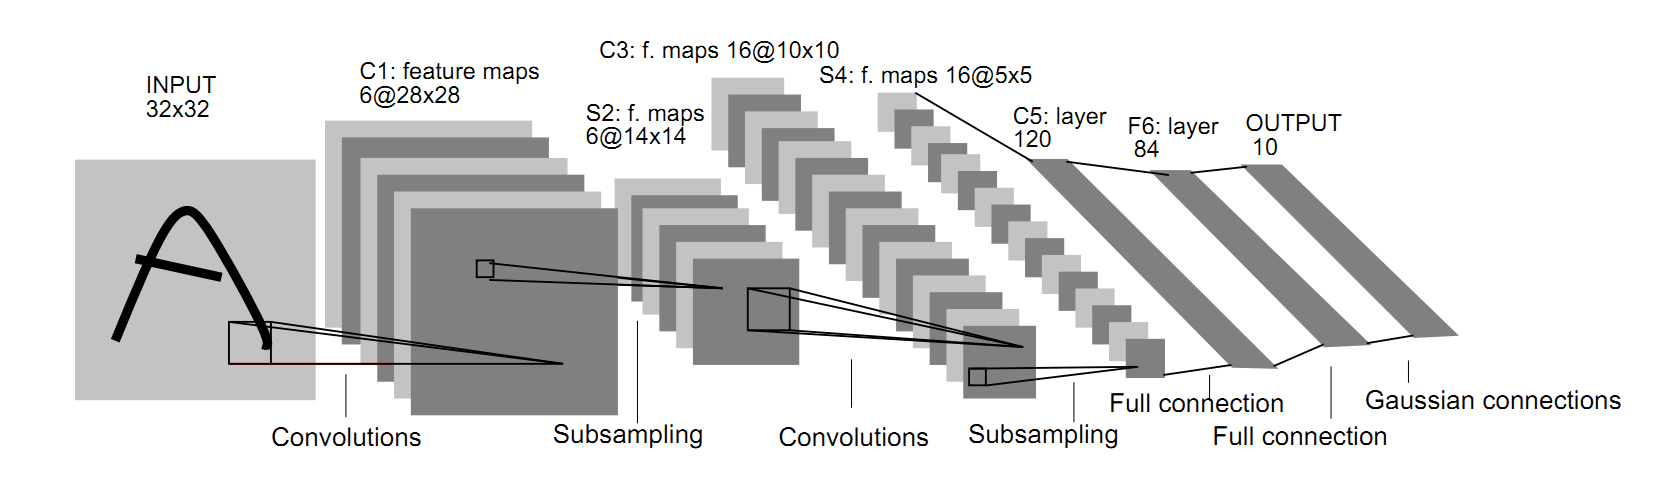
\includegraphics[width=14.5cm]{images/lenet-5.png}
    \caption{Konvolucijska neuronska mreža \emph{LeNet-5}, preuzeto iz \citep{Lecun1998}}
    \label{fig:lenet5}
\end{figure}

Kroz sljedećih nekoliko potpoglavlje bit će objašnjena uloga konvolucijskog sloja, sloja sažimanja te potpuno povezanoga sloja.

\section{Konvolucijski sloj}

Konvolucijski sloj, kako mu i ime govori, predstavlja jezgru same funkcionalnosti konvolucijske neuronske mreže. Svaki konvolucijski sloj se sastoji od filtra čije je težine potrebno podesiti to jest naučiti u fazi učenja neuronske mreže. Svaki filtar je predstavljen kao prostorna matrica dimenzija $w \times h \times d$ gdje $w$ označava širinu, $h$ visinu te $d$ dubinu filtra. Širina i visina filtra su najčešće manjih prostornih dimenzija od ulaza, dok je dubina filtra uvijek jednaka dubini ulaza. Na primjer, ukoliko se mreža koristi za klasificiranje slika u boji, točnije slika s tri komponente boja, tada bi dubina filtra bila tri, to jest filtar bi činile tri matrice dimenzije $w \times h$, odnosno jedna za svaku komponentu boje.

Izlaz konvolucijskog sloja predstavlja niz aktivacijskih mapa, to jest dvodimenzionalnih matrica. Pojedina aktivacijska mapa predstavlja odziv jednog filtra koja se dobiva tako što se filtar konvoluira s ulaznim prostorom. Konvoluiranje filtra s ulazom se može predstaviti kao pomicanje filtra za određeni korak po ulaznom prostoru te računanje skalarnog umnoška između težina filtra i vrijednosti ulaza za svaku poziciju. Prilikom učenja mreže težine filtra će se podesiti tako da se pojedini filtar ''aktivira'' na mjestima gdje uoči određene značajke poput rubova, nakupine boja pa čak i kružnih oblika u višim slojevima. Primjer konvolucije ulaza filtrom dan je na slici \ref{fig:conv_example} gdje prva matrica predstavlja ulazni prostor, druga filtar te zadnja aktivacijsku mapu.

\begin{figure}[htb]
    \centering
    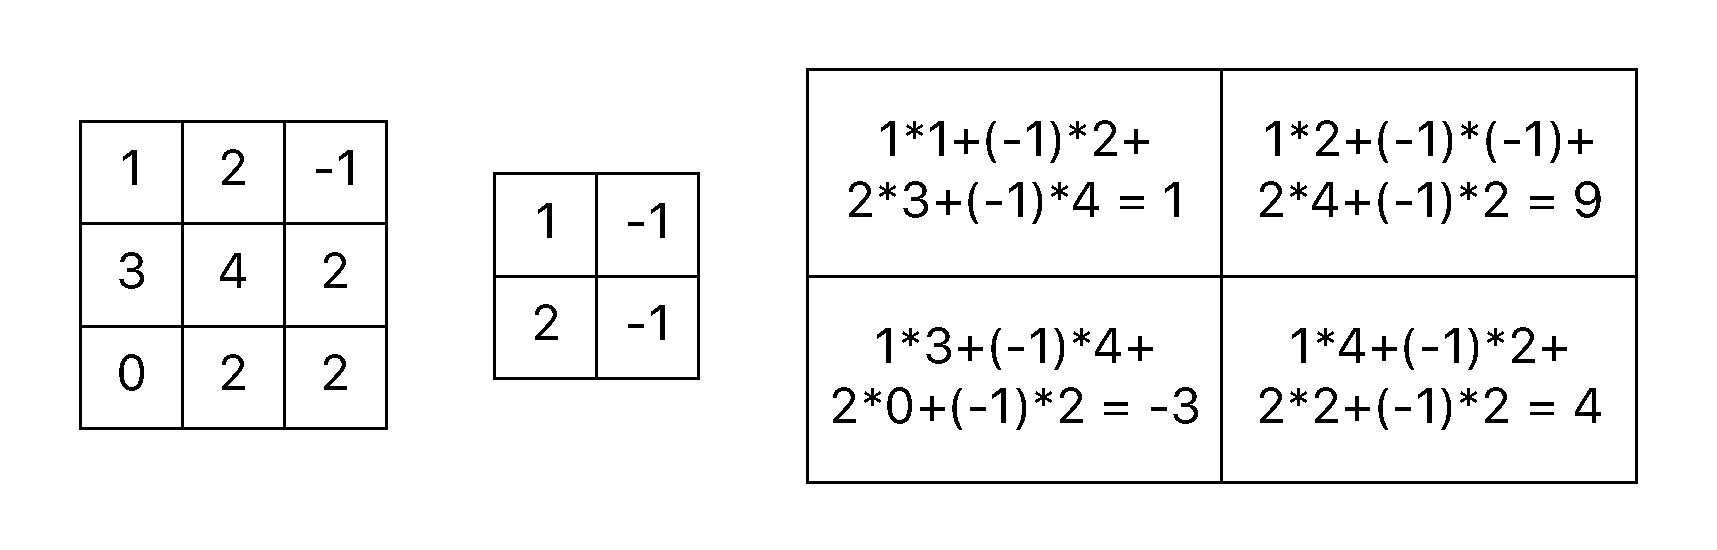
\includegraphics[width=14.5cm]{images/conv_example.pdf}
    \caption{Primjer konvolucije ulaza filtrom}
    \label{fig:conv_example}
\end{figure}

Veličina izlaza pojedinog konvolucijskog sloja definirana je s tri hiperparametara: brojem filtra, veličinom filtra te korakom pomaka filtra \engl{stride}. Korak pomaka filtra određuje za koliko koraka će se filtar pomicati po širini i visini ulaznog prostora u fazi konvolucije. Uz pretpostavku kvadratnoga filtra, da su mi širina i visina jednaki, što i je najčešći slučaj u praksi, veličina izlaza $W_o$ se može definirati izrazom \eqref{eq:conv_out}, gdje $W_i$ označava veličinu ulaza, $F$ veličinu filtra te $S$ korak pomaka filtra.
\begin{equation} \label{eq:conv_out}
W_o = \frac{W_i - F}{S} + 1
\end{equation}

Za razliku od potpuno povezanoga sloja, gdje je svaki izlaz spojen sa svim ulazima sljedećeg sloja, kod konvolucijskog sloja svaki izlaz je spojen samo sa malim dijelom ulaza sljedećeg sloja što dovodi do puno manje veza, a samim time i puno manje težina, to jest parametara koje je potrebno naučiti.

Često se u praksi izlazi konvolucijskog sloja, to jest vrijednosti aktivacijskih mapa, ''provlače'' kroz aktivacijsku funkciju danu izrazom \eqref{eq:relu}, koja se u literaturi naziva \emph{ReLU} \engl{rectified linear unit}.
\begin{equation} \label{eq:relu}
f(x) = max(0, x)
\end{equation}

\section{Sloj sažimanja}

Nakon jednog ili više konvolucijskih slojeva često dolazi i sloj sažimanja. Cilj navedenoga sloja je smanjenje prostornih dimenzija ulaza, odnosno aktivacijskih mapa. Smanjenjem prostornih dimenzija ulaza ovaj sloj zapravo kontrolira i smanjuje mogućnost prenaučenosti mreže jer povećava invarijantnost na pomak, to jest neosjetljivost na manje pomake značajki u ulaznom prostoru što je vrlo korisno u slučaju kada je za raspoznavanje bitnije utvrditi prisutnost određene značajke, nego njezinu točnu lokaciju.

U literaturi postoji nekoliko vrsti sažimanja: sažimanje srednjom vrijednosti, sažimanje maksimalnom vrijednosti, sažimanje L2 normom te sažimanje težinskim usrednjavanjem. U praksi se najčešće koristi sažimanje maksimalnom vrijednosti i to s filtrima dimenzija $2 \times 2$ koji ukupno odbacuju $75\%$ vrijednosti ulaza. Primjer takvog sažimanja dan je na slici \ref{fig:pool_example}.

\begin{figure}[htb]
    \centering
    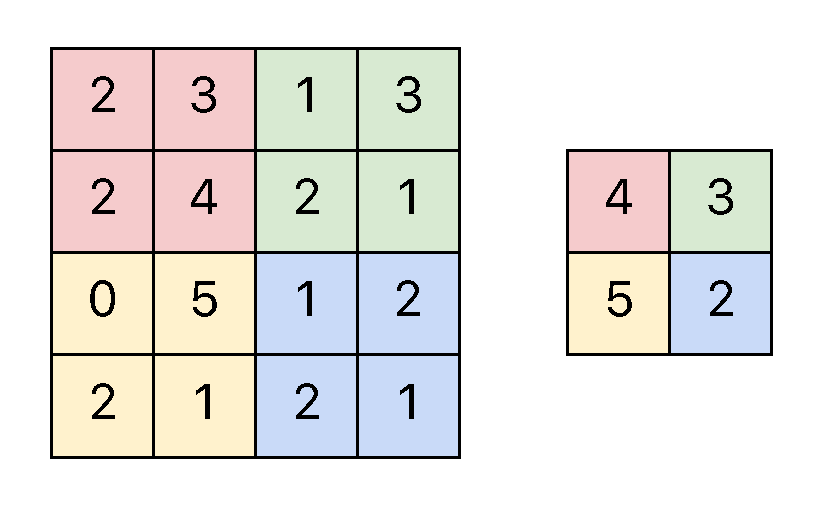
\includegraphics[width=7.5cm]{images/pool_example.pdf}
    \caption{Primjer sažimanja maksimalnom vrijednosti}
    \label{fig:pool_example}
\end{figure}

Bitno je uočiti kako sloj sažimanja utječe na smanjenje širine i visine ulaznog prostora, no ne i njegove dubine, to jest broja komponenti.

\section{Potpuno povezani sloj}

Kod potpuno povezanoga sloja ulaz pojedinog neurona je spojen s izlazima svih neurona iz prethodnog sloja te se sloj kao takav ne razlikuje onome iz obične neuronske mreže. Kod konvolucijskih neuronskih mreža jedan ili više potpuno povezanih slojeva dolaze na samom kraju mreže te njihova uloga je sama klasifikacija. Stoga, konvolucijske mreže se mogu rastaviti na dva dijela: prvi dio čine konvolucijski slojevi te slojevi sažimanja, a drugi dio potpuno povezani slojevi. Prvi dio mreže se može promatrati kao sustav za izlučivanje značajki, dok se drugi dio može promatrati kao obična neuronska mreža, to jest klasifikator.